\documentclass[a4paper,francais]{article}
\usepackage[utf8]{inputenc}
\usepackage[T1]{fontenc}
\usepackage[french]{babel}

\usepackage{subfig}
\usepackage{graphicx}
\graphicspath{{fig/}}
\newcommand{\caserne}{\begin{picture}(0,0) \put(255,100){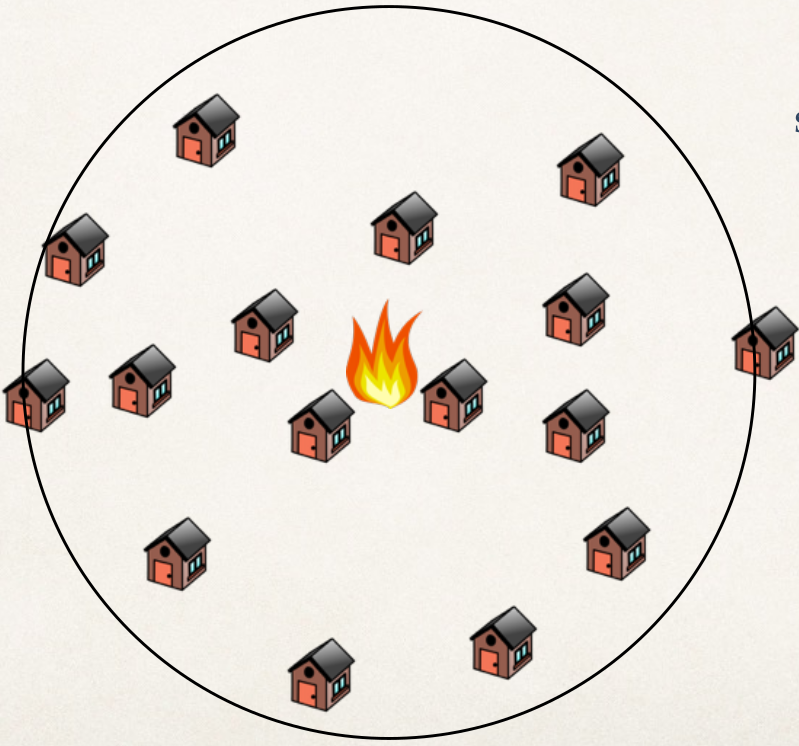
\includegraphics[width=25mm]{caserne}} \end{picture}}

\usepackage{amsmath}
\usepackage{amssymb}
\usepackage{amsthm}
\usepackage{cancel}
\usepackage{enumitem}

\usepackage{hyperref}

\usepackage{cprotect} %verbatim in footnote

\newcommand{\cad}{c.-à-d.}
\newcommand{\Z}{{\ensuremath\mathbb{Z}}}
\newcommand{\N}{{\ensuremath\mathbb{N}}}
\newcommand{\R}{{\ensuremath\mathbb{R}}}
\newtheorem{Theorem}{Theorem}
\newtheorem{Exemple}{Exemple}

%-------- enable or disable correction -----------------------------
\theoremstyle{definition}
\newtheorem{exercice}{Exercice}[section]
\newtheorem*{solution}{Solution}

\usepackage{comment}
\excludecomment{solution}% commenter/décommenter pour afficher/effacer l'impression des solutions

\let\vec\mathbf

\title{Où placer les pompiers ? \\ \large Résoudre un problème d'optimisation convexe}
\author{Tristan Roussillon}

\begin{document}

\maketitle
\caserne

\section{Introduction}

Nous nous intéressons au problème suivant : étant donné un ensemble $E$ de points dans le plan, 
trouver le plus petit disque contenant $E$. C'est un problème simple à comprendre, qui a 
toujours une solution unique et qui a des applications variées (localisation optimale, 
apprentissage automatique, vision par ordinateur, informatique graphique, etc.). 
De nombreux algorithmes combinatoires existent pour ce problème, mais nous allons le résoudre
numériquement, à l'aide de la méthode de Frank et Wolfe.

\section{Formulation du problème et dualité}

\'Etant donné un ensemble de $n$ points du plan $\{(x_i, y_i)\}_{i = 1, \dots, n}$,
nous considérons le problème d'optimisation sous contrainte suivant :
\[
\text{(P)}
\left\{
\begin{array}{ll}
  \min \ r^2 \\
  \text{sujet aux contraintes :} \\
  \forall i = 1, \dots, n, \ (x_i - c_x)^2 + (y_i - c_y)^2 \leq r^2 \\ 
  c_x, c_y, r \in \R \\
\end{array}
\right.
\]

\begin{exercice}
  Donnez une interprétation géométrique des variables $c_x, c_y, r$ et expliquez en quoi
  le problème (P) est une formalisation correcte du problème énoncé en introduction.
\end{exercice}

En théorie de l'optimisation, la dualité désigne le principe selon lequel les problèmes
d'optimisation peuvent être vus de deux perspectives, le problème de départ, appelé
\emph{primal}, ou son problème \emph{dual} dont la solution est, sous certaines conditions,
notamment la convexité du problème primal, \emph{égale} à la solution du problème primal. 

Nous allons maintenant considérer le problème dual suivant\footnote{Comment le problème dual a été
  déduit du problème primal est au-delà du périmètre du cours.} :
\[
\text{(D)}
\left\{
\begin{array}{l}
  \min_{\vec{u}} \ \phi(\vec{u}) :=
  \sum_i^n\sum_j^n \vec{u}_i\vec{u}_j (x_ix_j + y_iy_j) - \sum_i^n \vec{u}_i (x_i^2 + y_i^2) \\
  \text{sujet aux contraintes :} \\
  \vec{u} \in \R^n, \|\vec{u}\|_1 = 1 \ \text{et} \ \forall i = 1, \dots, n, \  \vec{u}_i \geq 0 \\
\end{array}
\right.
\]

Nous avons la propriété suivante : si $\vec{u}^\star$ est une solution optimale de (D),
alors le plus petit disque recouvrant les points $\{(x_i, y_i)\}_{i = 1, \dots, n}$ est
de centre $\sum_i^n \vec{u}^\star_i (x_i, y_i)$ et de rayon $\sqrt{-\phi(\vec{u}^\star)}$. 

\begin{exercice}
  Expliquez pourquoi (D) est un problème d'optimisation convexe sous contraintes linéaires.
  Soyez plus ou moins formel en fonction de vos capacités en mathématique. 
\end{exercice}



%% \begin{exercice}
%%   \`A l'aide du changement de variable $\rho :=c_x^2 + c_y^2 - r^2$, reformulez (P) en un
%%   problème (P') ayant une fonction objective sous la forme d'un polynôme de degré 2 et
%%   des contraintes linéaires.
%%   %sous la forme de combinaisons linéaires des variables inférieures à une constante.
%%   Piste : mettre au carré, développer l'inégalité, opérer le changement de variable.
%%   Faites valider par l'enseignant. 
%% \end{exercice}

%% \begin{solution}
%% \[
%% \text{(P')}
%% \left\{
%% \begin{array}{ll}
%%   \min_{c_x, c_y, \rho} \ c_x^2 + c_y^2 - \rho \ \text{tel que} & \\
%%   (-2x_i) c_x + (-2y_i) c_y + \rho  \leq -(x_i^2 + y_i^2) & \forall i = 1, \dots, n \\ 
%%   c_x, c_y, \rho \in \R \\
%% \end{array}
%% \right.
%% \]
%% \end{solution}

%% \begin{exercice}
%%   Calculez le gradient et le hessien de la fonction objective de (P').
%%   Calculez les trois valeurs propres du hessien\footnote{Vous pouvez
%%     vérifier avec \url{http://www.arndt-bruenner.de/mathe/scripts/engl_eigenwert2.htm}}.
%%   Déduisez-en que c'est une matrice semi-définie positive et que la fonction est convexe. 
%% \end{exercice}

%% \begin{solution}
%%   Le hessien de la fonction objective notée $f$ est
%%   \[
%%     {\nabla^2f}(c_x,c_y,\rho) =
%%     \begin{pmatrix}
%%       2 & 0 & 0 \\
%%       0 & 2 & 0 \\
%%       0 & 0 & 0 \\
%%     \end{pmatrix}
%%   \]
%%   Il est constant et noté plus simplement $H$.
  
%%   Ses valeurs propres sont les valeurs $\lambda(\lambda_1, \lambda_2, \lambda_3)$
%%   vérifiant $\det{(\lambda I - H)} = 0$. En développant le déterminant, on obtient
%%   l'égalité $\lambda_3(\lambda_1 - 2)(\lambda_2 - 2) = 0$, ce qui signifie que les
%%   valeurs propres sont $2, 2$ et $0$, toutes positives, d'où l'on déduit que
%%   H est semi-définie positive, et par suite, comme le hessien de $f$ l'est partout,
%%   que $f$ est convexe. 
%% \end{solution}

\section{Résolution numérique de (D) en python}

Dans cette section, votre objectif est d'écrire un programme python pour résoudre (D)
à l'aide de la méthode de Frank et Wolfe
\footnote{Lire \url{https://en.wikipedia.org/wiki/Frank\%E2\%80\%93Wolfe_algorithm}}. 

\begin{exercice}
  \'Ecrivez un script python qui génère aléatoirement un ensemble de $100$ points se trouvant
  dans le cercle de centre $(100,100)$ et de rayon $100$. Utilisez un moyen à votre convenance
  pour afficher les points et le cercle solution (matplotlib, svg, etc.)   
\end{exercice}

\begin{exercice}
  \'Ecrivez le code permettant de résoudre (D) selon la méthode de Frank et Wolfe en fixant
  arbitrairement le nombre d'étapes à 50.
  
  \`A chaque étape, vous devez utiliser un solveur d'optimisation linéaire, soit
  \href{https://docs.scipy.org/doc/scipy-1.3.3/reference/generated/scipy.optimize.linprog.html#scipy.optimize.linprog}{\texttt{linprog}}, 
  soit \href{https://docs.scipy.org/doc/scipy-1.3.3/reference/generated/scipy.optimize.minimize.html}{\texttt{minimize}}.
  (Vous aurez aussi certainement besoin de
  \href{https://docs.scipy.org/doc/numpy/reference/routines.array-creation.html}{créer} et
  \href{https://docs.scipy.org/doc/numpy/reference/routines.array-manipulation.html}{manipuler} des
  tableaux
  \href{https://numpy.org/doc/stable/contents.html#numpy-docs-mainpage}{\texttt{NumPy}}
  et vous pouvez bien sûr vous inspirer des programmes corrigés donnés précédemment).
  
  Pour l'initialisation, vous pouvez choisir un vecteur dont la première coordonnée est fixée à $1$
  et toutes les autres à $0$.

  Le plus dur sera de calculer le gradient de $\phi$. N'hésitez pas à vous faire aider sur ce point. 
\end{exercice}

\begin{solution}
  Note:
  \[
  \frac{\partial \phi(\vec{u})}{\partial \vec{u}_k} =
  (2\vec{u}_k - 1)(x_k^2+y_k^2) + 2 \sum_{i, i \neq k}^n \vec{u}_i (x_kx_i + y_ky_j)
  \]
\end{solution}

\begin{exercice}
  Expliquez pourquoi la solution que vous obtenez à chaque étape de l'algorithme de Frank et Wolfe est
  un vecteur ayant une coordonnée à $1$ et toutes les autres à $0$. 
\end{exercice}

\begin{exercice}
  Expliquez pourquoi le cercle solution que vous obtenez n'englobe pas forcément tous les points mais presque.
\end{exercice}

\section{Bonus}

\begin{exercice}
  Lisez les sections 1.1 et 2 de \cite{yildirim} et implémentez l'algorithme 3.1. 
\end{exercice}

\begin{thebibliography}{1}

\bibitem{yildirim}
E.~Alper Yildirim.
\newblock \href{http://www.optimization-online.org/DB_FILE/2007/05/1654.pdf}{Two algorithms for the minimum enclosing ball problem}.
\newblock {\em SIAM J. on Optimization}, 19(3):1368–1391, nov 2008.

\end{thebibliography}

\end{document}


